%
% main.tex
%
% Copyright (C) 2022 by SpaceLab.
%
% Camera Payload Preliminary Design Review
%
% This work is licensed under the Creative Commons Attribution-ShareAlike 4.0
% International License. To view a copy of this license,
% visit http://creativecommons.org/licenses/by-sa/4.0/.
%

%
% \brief Main file.
%
% \author Gabriel Mariano Marcelino <gabriel.mm8@gmail.com>
% \author Vitória Beatriz Bianchin <vitoriabbianchin@gmail.com>
% \author Caique Sales de Miranda Gomes <kiqsmg@gmail.com>
%
% \version 0.1.0
%
% \date 2022/06/24
%

\documentclass{beamer}

\usepackage{presentation}

\title[Presentation]{SpaceLab Camera Payload (SLCam) - PDR}
\author[SpaceLab]{Vitória B. Bianchin, Caique S. de Miranda Gomes, Gabriel M. Marcelino}
\institute[]{SpaceLab - UFSC}
\date{2022 July 20}

\hypersetup
{
    pdfauthor	= {SpaceLab},
    pdfsubject	= {Preliminary design review (PDR) of the camera payload},
    pdftitle	= {\title},
    pdfkeywords	= {Nanosatellites, CubeSats, Payload, Camera}
}

\begin{document}

    %
% \brief Title page.
%
% \author Gabriel Mariano Marcelino <gabriel.mm8@gmail.com>
%
% \version 0.2.0
%
% \date 2023/02/09
%

\begin{titlepage}

\thispagestyle{empty}

\begin{flushleft}
SLB-CAM-DOC-v0.2
\end{flushleft}

\vspace{1cm}

\begin{figure}[!ht]
    \begin{flushleft}
        
\includegraphics[width=7cm]{figures/spacelab-logo-full-color-rgb-1000px@72ppi.png}
    \end{flushleft}
\end{figure}

\begin{flushleft}
\Huge{\textbf{\thetitle}}
\rule[0pt]{\textwidth}{5pt}
\end{flushleft}

\vspace{0.2cm}

\begin{flushleft}
\textit{\thetitle} \\
\textit{SpaceLab, Universidade Federal de Santa Catarina, Florianópolis - Brazil}
\end{flushleft}

\vfill
\vfill

\begin{flushright}
April 2023
\end{flushright}

\end{titlepage}

    %
% contents.tex
%
% Copyright (C) 2022 by SpaceLab.
%
% Camera Payload Preliminary Design Review
%
% This work is licensed under the Creative Commons Attribution-ShareAlike 4.0
% International License. To view a copy of this license,
% visit http://creativecommons.org/licenses/by-sa/4.0/.
%

%
% \brief Table of contents.
%
% \author Gabriel Mariano Marcelino <gabriel.mm8@gmail.com>
% \author Vitória Beatriz Bianchin <vitoriabbianchin@gmail.com>
% \author Caique Sales de Miranda Gomes <kiqsmg@gmail.com>
%
% \version 0.1.0
%
% \date 2022/06/24
%

\begin{frame}
    \frametitle{Summary}
    \tableofcontents
\end{frame}


    \section{Project Overview}

        %
% introduction.tex
%
% Copyright (C) 2022 by SpaceLab.
%
% Camera Payload Preliminary Design Review
%
% This work is licensed under the Creative Commons Attribution-ShareAlike 4.0
% International License. To view a copy of this license,
% visit http://creativecommons.org/licenses/by-sa/4.0/.
%

%
% \brief Introduction slides.
%
% \author Gabriel Mariano Marcelino <gabriel.mm8@gmail.com>
% \author Vitória Beatriz Bianchin <vitoriabbianchin@gmail.com>
% \author Caique Sales de Miranda Gomes <kiqsmg@gmail.com>
%
% \version 0.1.0
%
% \date 2022/06/24
%

\begin{frame}{Proposal and Objectives}

    \begin{columns}[t]
        \begin{column}[t]{0.6\textwidth}
            \begin{itemize}
                \item Camera payload for small satellites (CubeSats)
                \vspace{0.5cm}
                \item Project name: ``\textit{SLCam}'' (SpaceLab Camera)
                \vspace{0.5cm}
                \item Main objective: Take pictures of the Earth from space
            \end{itemize}
        \end{column}
        \begin{column}[t]{0.4\textwidth}
            \begin{figure}[!ht]
                \begin{center}
                    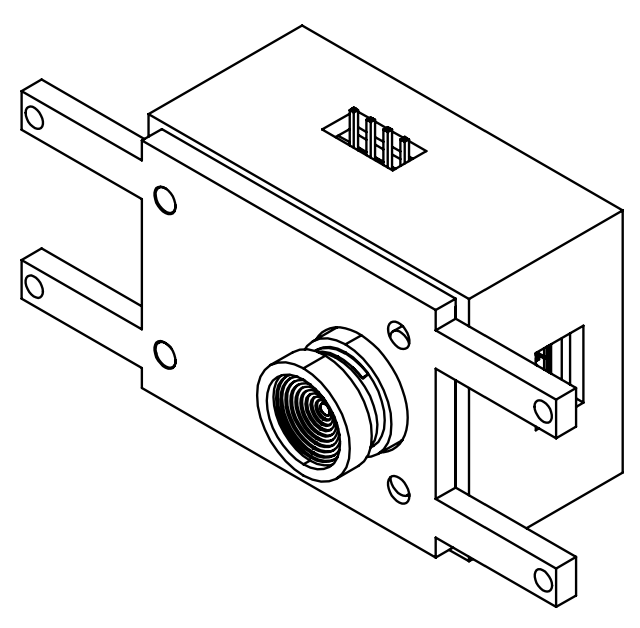
\includegraphics[width=4cm]{figures/slcam-dw}
                \end{center}
            \end{figure}
        \end{column}
    \end{columns}

\end{frame}

    \section{Related Projects and References}

        %
% related-work.tex
%
% Copyright (C) 2022 by SpaceLab.
%
% Camera Payload Preliminary Design Review
%
% This work is licensed under the Creative Commons Attribution-ShareAlike 4.0
% International License. To view a copy of this license,
% visit http://creativecommons.org/licenses/by-sa/4.0/.
%

%
% \brief Introduction slides.
%
% \author Gabriel Mariano Marcelino <gabriel.mm8@gmail.com>
% \author Vitória Beatriz Bianchin <vitoriabbianchin@gmail.com>
% \author Caique Sales de Miranda Gomes <kiqsmg@gmail.com>
%
% \version 0.1.0
%
% \date 2022/06/24
%


\begin{frame}{Comercial Cameras for CubeSats}

    A few commercial camera modules for CubeSats are available in the market:

    \begin{itemize}
        \item \href{https://gomspace.com/shop/payloads/earth-observation.aspx}{\textcolor{blue}{\underline{GomSpace NanoCam C1U}}}
        \vspace{0.4cm}
        \item \href{https://www.skyfoxlabs.com/product/27-digital-cubesat-camera}{\textcolor{blue}{\underline{SkyFox Labs piCAM}}}
        \vspace{0.4cm}
        \item \href{https://www.aac-clyde.space/what-we-do/space-products-components/payloads/im200}{\textcolor{blue}{\underline{AAC Hyperion IM200}}}
        \vspace{0.4cm}
        \item \href{https://redwirespace.com/products/spectracam}{\textcolor{blue}{\underline{RedWire SpectraCAM}}}
        \vspace{0.4cm}
        \item \href{https://dragonflyaerospace.com/products/gecko/}{\textcolor{blue}{\underline{Dragonfly Gecko Imager}}}
    \end{itemize}

\end{frame}

% #########################################################################
% #########################################################################

\begin{frame}{Comercial Cameras for CubeSats: \href{https://gomspace.com/shop/payloads/earth-observation.aspx}{\textcolor{cyan}{\underline{GomSpace NanoCam C1U}}}}

    \begin{columns}[t]
        \begin{column}[t]{0.6\textwidth}
            \begin{itemize}
                \item Res.: 3 MP (2048 $\times$ 1536 px)
                \item Sensor: Aptina MT9T031 (1/2'' CMOS)
                \item Lens: 8, 35 or 70 mm
                \item Processing:
                    \begin{itemize}
                        \item Processor: ARM
                        \item Memory: 512 MB RAM/2 GB flash
                    \end{itemize}
                \item Interfaces: CAN/I$^{2}$C
                \item Dimensions: 96 $\times$ 90 mm (PC104)
                \item Mass: 169 to 277 g
            \end{itemize}
        \end{column}
        \begin{column}[t]{0.4\textwidth}
            \vspace{0.7cm}
            \begin{figure}[!ht]
                \begin{center}
                    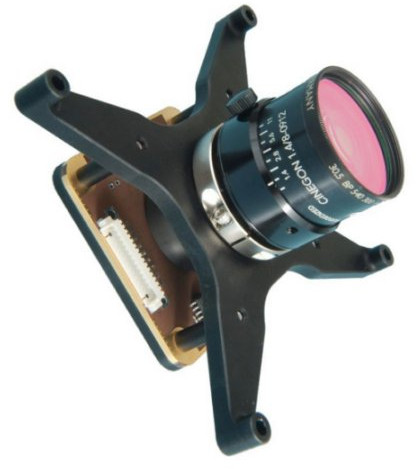
\includegraphics[width=4cm]{figures/nanocamc1u}
                \end{center}
            \end{figure}
        \end{column}
    \end{columns}

\end{frame}

% #########################################################################
% #########################################################################

\begin{frame}{Comercial Cameras for CubeSats: \href{https://gomspace.com/shop/payloads/earth-observation.aspx}{\textcolor{cyan}{\underline{GomSpace NanoCam C1U}}}}

\textcolor{blue}{PROCURAR FOTOS TIRADAS POR ESSE MÓDULO!!!}

\end{frame}

% #########################################################################
% #########################################################################

\begin{frame}{Comercial Cameras for CubeSats: \href{https://www.skyfoxlabs.com/product/27-digital-cubesat-camera}{\textcolor{cyan}{\underline{SkyFox Labs piCAM}}}}

    \begin{columns}[t]
        \begin{column}[t]{0.65\textwidth}
            \begin{itemize}
                \item Res.: VGA (640 $\times$ 480 px)
                \item Sensor: Color RGB
                \item Lens: 76$^{\circ}$ (default), 116$^{\circ}$ or 170$^{\circ}$ (FoV)
                \item Interface: UART (115200 bps) 
                \item Consumption: 315 mW (typical)
                \item Dimensions: 48 $\times$ 33 $\times$ 40,5 mm
                \item Mass: 40 g
                \item Price: 4390 EUR (FM)
            \end{itemize}
        \end{column}
        \begin{column}[t]{0.35\textwidth}
            \begin{figure}[!ht]
                \begin{center}
                    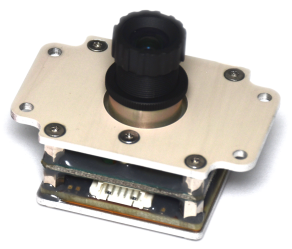
\includegraphics[width=3.5cm]{figures/picam-front}
                \end{center}
            \end{figure}
            \begin{figure}[!ht]
                \begin{center}
                    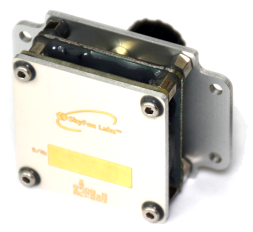
\includegraphics[width=3.5cm]{figures/picam-back}
                \end{center}
            \end{figure}
        \end{column}
    \end{columns}
    
\end{frame}

% #########################################################################
% #########################################################################

\begin{frame}{Comercial Cameras for CubeSats: \href{https://www.skyfoxlabs.com/product/27-digital-cubesat-camera}{\textcolor{cyan}{\underline{SkyFox Labs piCAM}}}}

    \begin{itemize}
        \item Examples (lens: 76$^{\circ}$, with IR-filter):
    \end{itemize}
    \begin{figure}[!ht]
        \begin{center}
            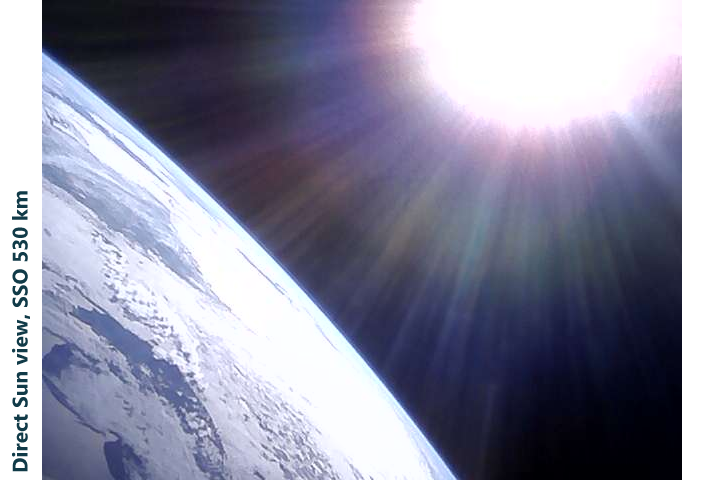
\includegraphics[width=9cm]{figures/picam-ex1}
        \end{center}
    \end{figure}

\end{frame}

\begin{frame}{Comercial Cameras for CubeSats: \href{https://www.skyfoxlabs.com/product/27-digital-cubesat-camera}{\textcolor{cyan}{\underline{SkyFox Labs piCAM}}}}

    \begin{figure}[!ht]
        \begin{center}
            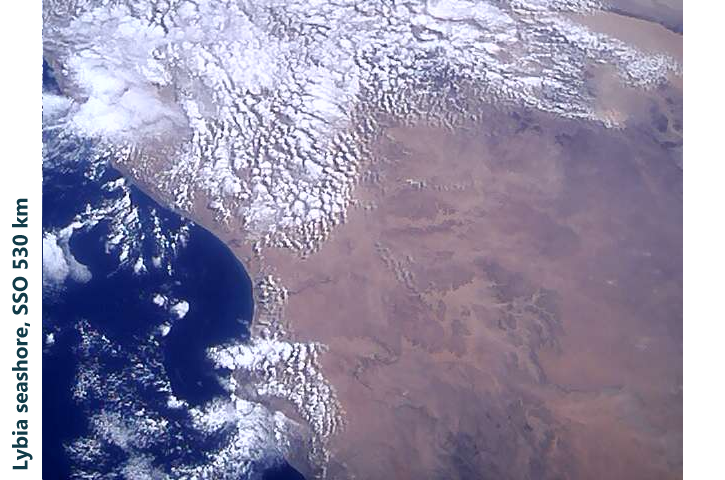
\includegraphics[width=10cm]{figures/picam-ex2}
        \end{center}
    \end{figure}

\end{frame}

\begin{frame}{Comercial Cameras for CubeSats: \href{https://www.skyfoxlabs.com/product/27-digital-cubesat-camera}{\textcolor{cyan}{\underline{SkyFox Labs piCAM}}}}

    \begin{figure}[!ht]
        \begin{center}
            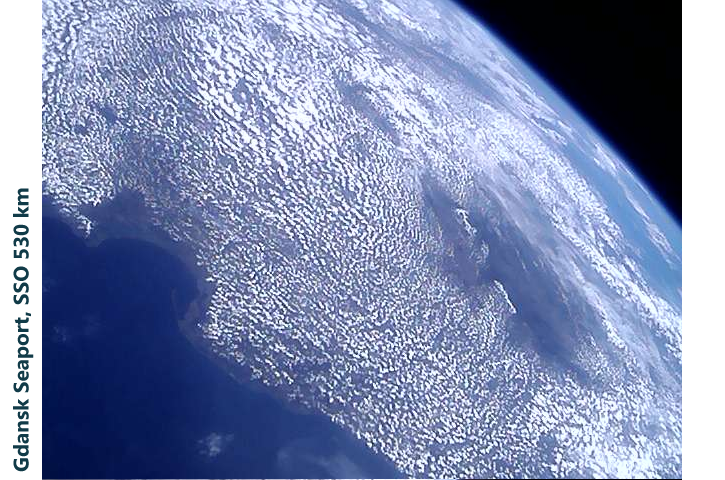
\includegraphics[width=10cm]{figures/picam-ex3}
        \end{center}
    \end{figure}

\end{frame}

% #########################################################################
% #########################################################################

\begin{frame}{Custom Projects}

    Some custom projects can also be found, like:

    \begin{itemize}
        \item .
        \item ...
    \end{itemize}

\end{frame}

% #########################################################################
% #########################################################################

\begin{frame}{Custom Projects: \href{http://www.madeinepal.com/2016/03/complete-guide-to-designing-camera.html}{\textcolor{cyan}{\underline{SNUSat}}}}

    \begin{columns}[t]
        \begin{column}[t]{0.6\textwidth}
            \begin{itemize}
                \item .
            \end{itemize}
        \end{column}
        \begin{column}[t]{0.5\textwidth}
            \begin{figure}[!ht]
                \begin{center}
                    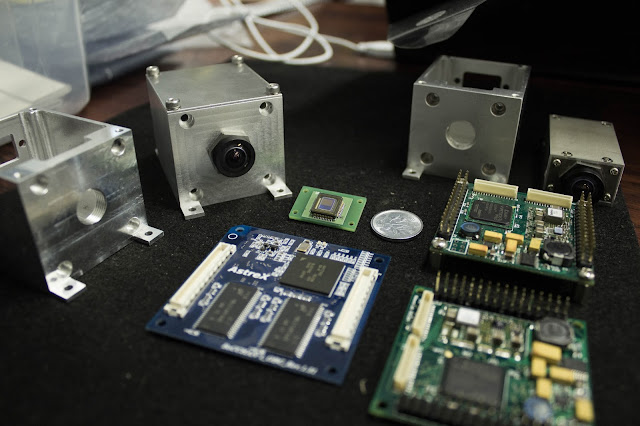
\includegraphics[width=5cm]{figures/snucam}
                \end{center}
            \end{figure}
        \end{column}
    \end{columns}

\end{frame}

% #########################################################################
% #########################################################################

\begin{frame}{Custom Projects: \href{http://stf1.com/}{\textcolor{cyan}{\underline{STF-1}}}}

    \begin{columns}[t]
        \begin{column}[t]{0.6\textwidth}
            \begin{itemize}
                \item Image sensor module: ArduCam Mini 2MP Plus
                \item ...
            \end{itemize}
        \end{column}
        \begin{column}[t]{0.4\textwidth}
            \begin{figure}[!ht]
                \begin{center}
                    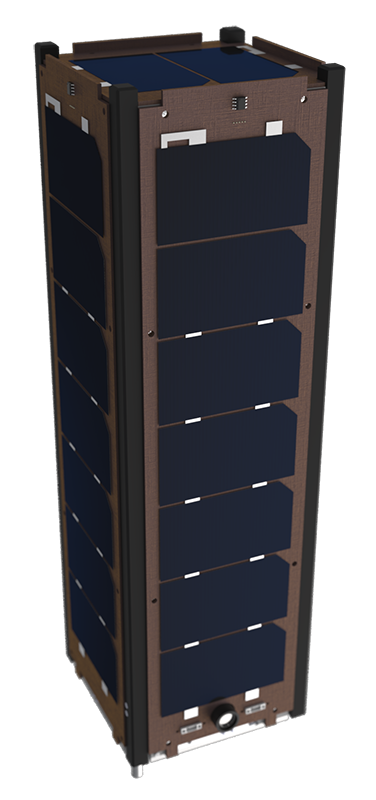
\includegraphics[width=3cm]{figures/stf1_closed_top.png}
                \end{center}
            \end{figure}
        \end{column}
    \end{columns}

\end{frame}

\begin{frame}{Custom Projects: \href{http://stf1.com/}{\textcolor{cyan}{\underline{STF-1}}}}

    \begin{columns}[t]
        \begin{column}[t]{0.4\textwidth}
            \begin{figure}[!ht]
                \begin{center}
                    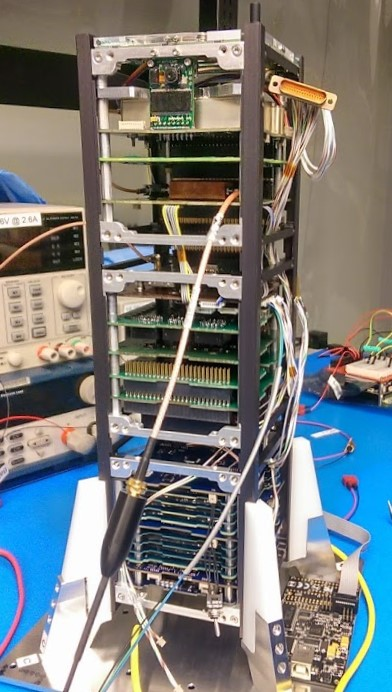
\includegraphics[width=3.5cm]{figures/stf1_integration-2.jpg}
                \end{center}
            \end{figure}
        \end{column}
        \begin{column}[t]{0.6\textwidth}
            \begin{figure}[!ht]
                \begin{center}
                    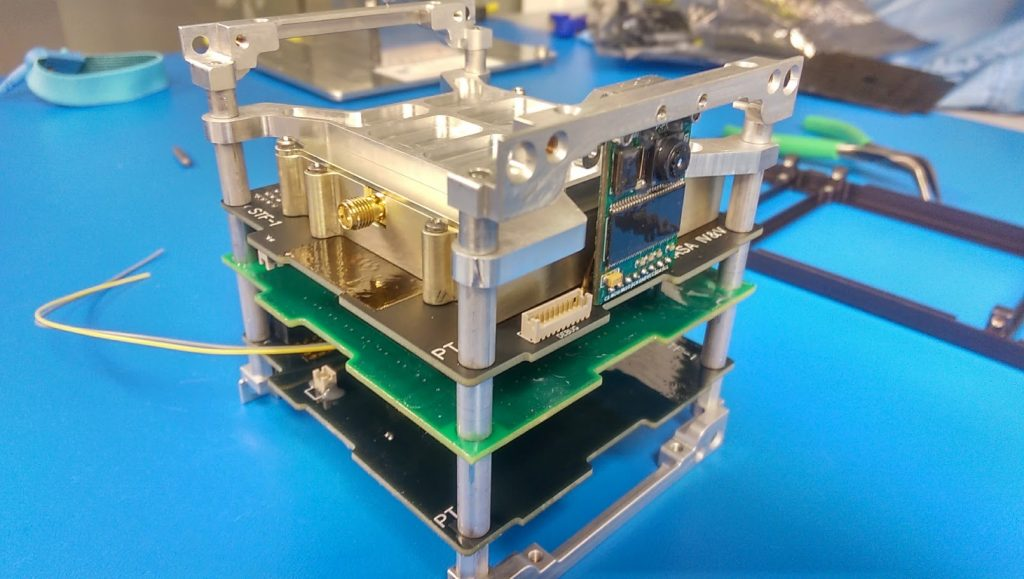
\includegraphics[width=5.5cm]{figures/stf1_stack_top-1024x579.jpg}
                \end{center}
            \end{figure}
            \begin{figure}[!ht]
                \begin{center}
                    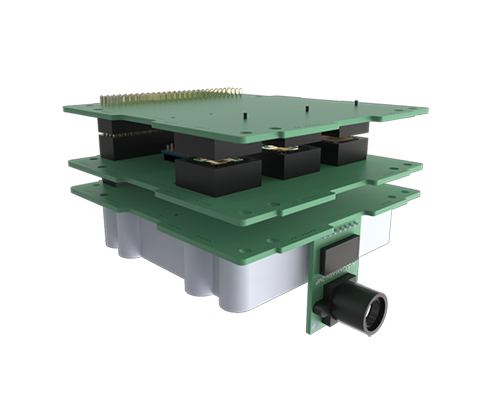
\includegraphics[width=4.5cm]{figures/stf1_bottom_cube.png}
                \end{center}
            \end{figure}
        \end{column}
    \end{columns}

\end{frame}

\begin{frame}{Custom Projects: \href{http://stf1.com/}{\textcolor{cyan}{\underline{STF-1}}}}

    \begin{figure}[!ht]
        \begin{center}
            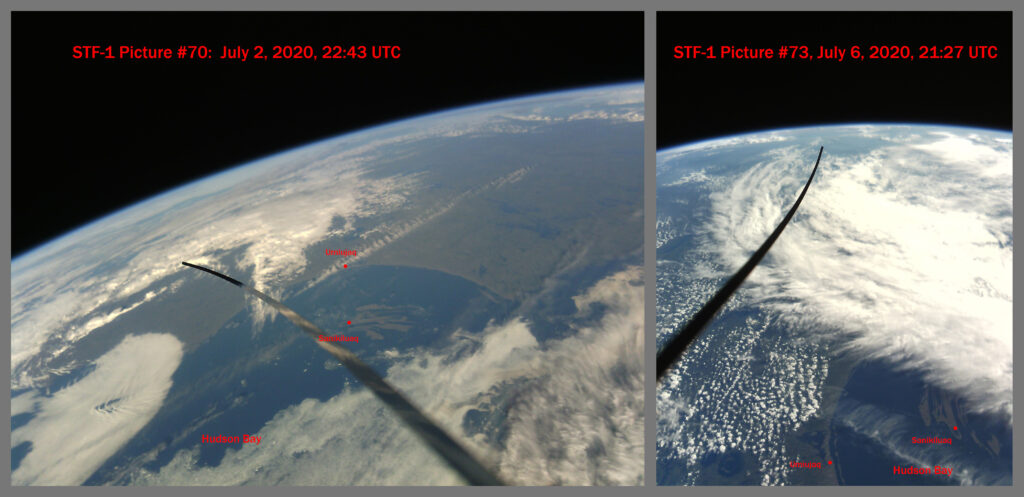
\includegraphics[width=10.5cm]{figures/stf-1-ex1.jpg}
        \end{center}
    \end{figure}

\end{frame}

\begin{frame}{Custom Projects: \href{http://stf1.com/}{\textcolor{cyan}{\underline{STF-1}}}}

    \begin{figure}[!ht]
        \begin{center}
            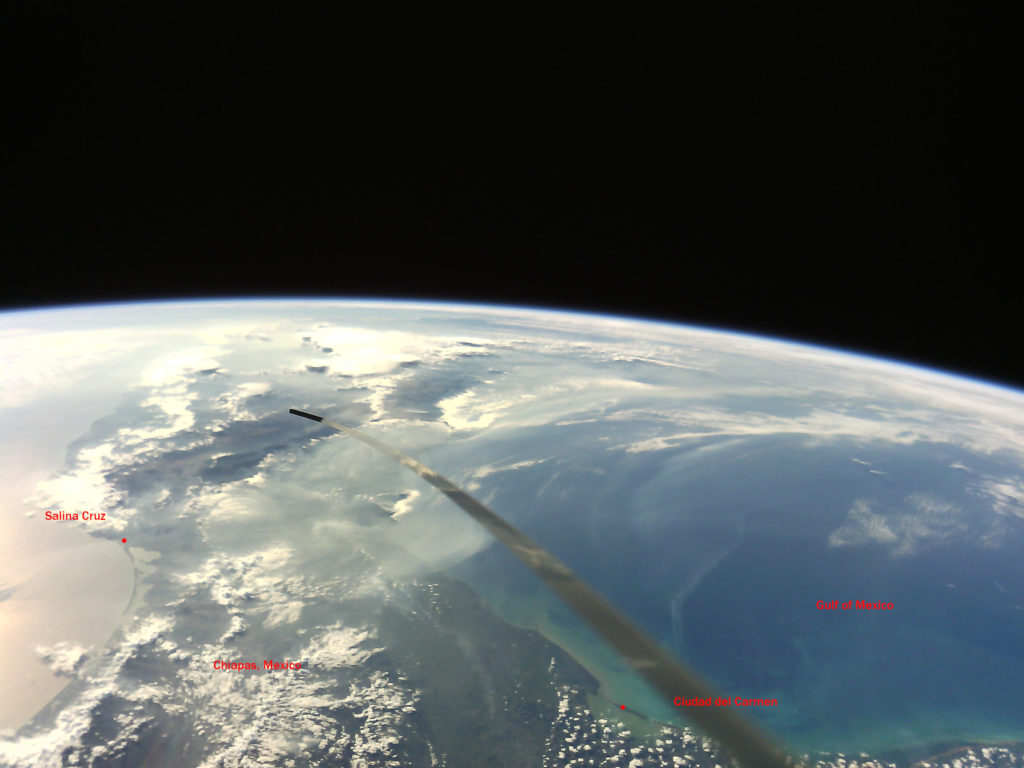
\includegraphics[width=9.5cm]{figures/stf-1-ex2.jpg}
        \end{center}
    \end{figure}

\end{frame}

\begin{frame}{Custom Projects: \href{http://stf1.com/}{\textcolor{cyan}{\underline{STF-1}}}}

    \begin{figure}[!ht]
        \begin{center}
            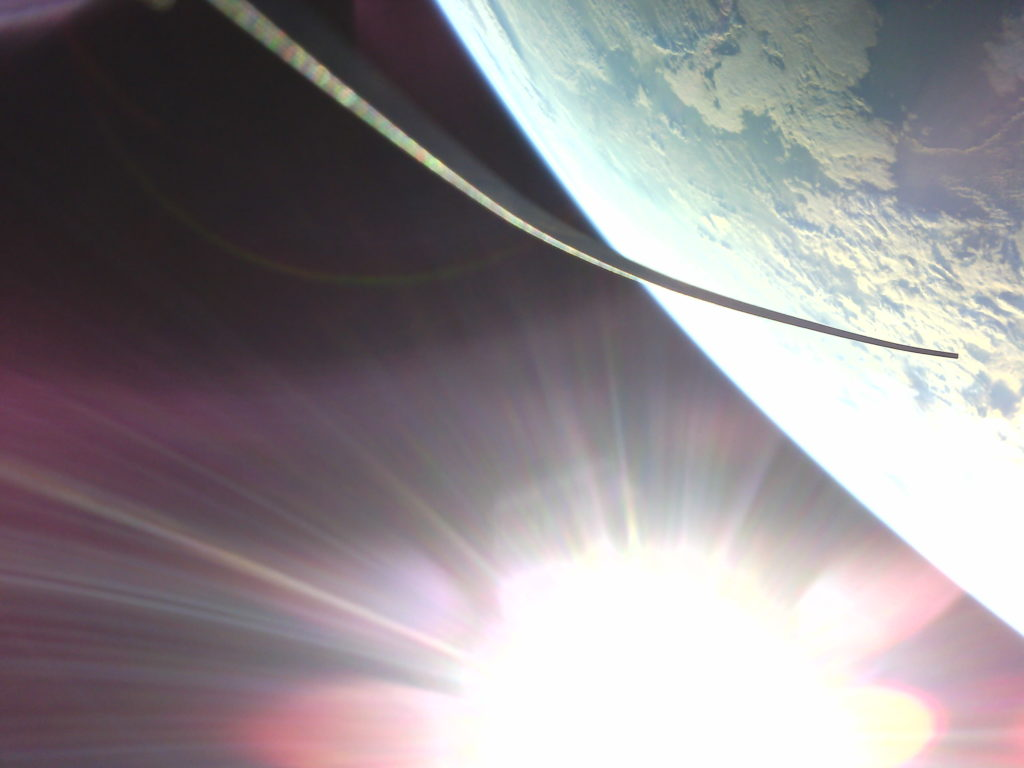
\includegraphics[width=9.5cm]{figures/stf-1-ex3.jpg}
        \end{center}
    \end{figure}

\end{frame}

\begin{frame}{Custom Projects: \href{http://stf1.com/}{\textcolor{cyan}{\underline{STF-1}}}}

    \begin{figure}[!ht]
        \begin{center}
            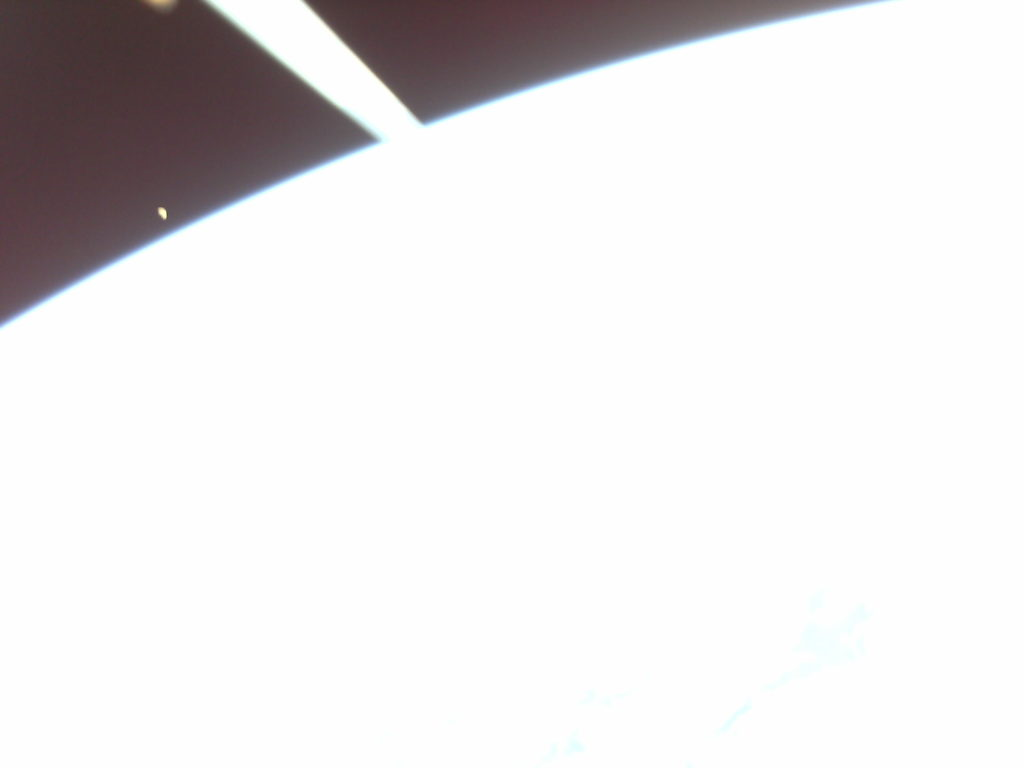
\includegraphics[width=9.5cm]{figures/stf-1-ex4.jpg}
        \end{center}
    \end{figure}

\end{frame}

\begin{frame}{Custom Projects: \href{http://stf1.com/}{\textcolor{cyan}{\underline{STF-1}}}}

    \begin{figure}[!ht]
        \begin{center}
            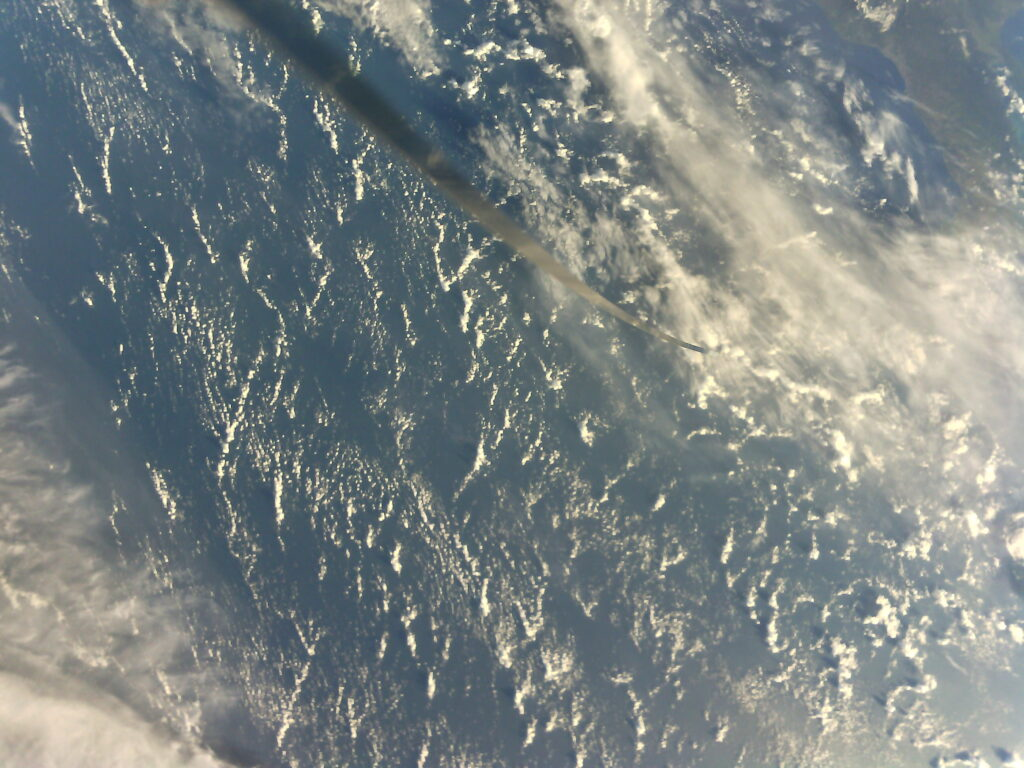
\includegraphics[width=9.5cm]{figures/stf-1-ex5.jpg}
        \end{center}
    \end{figure}

\end{frame}

\begin{frame}{Custom Projects: \href{http://stf1.com/}{\textcolor{cyan}{\underline{STF-1}}}}

    \begin{figure}[!ht]
        \begin{center}
            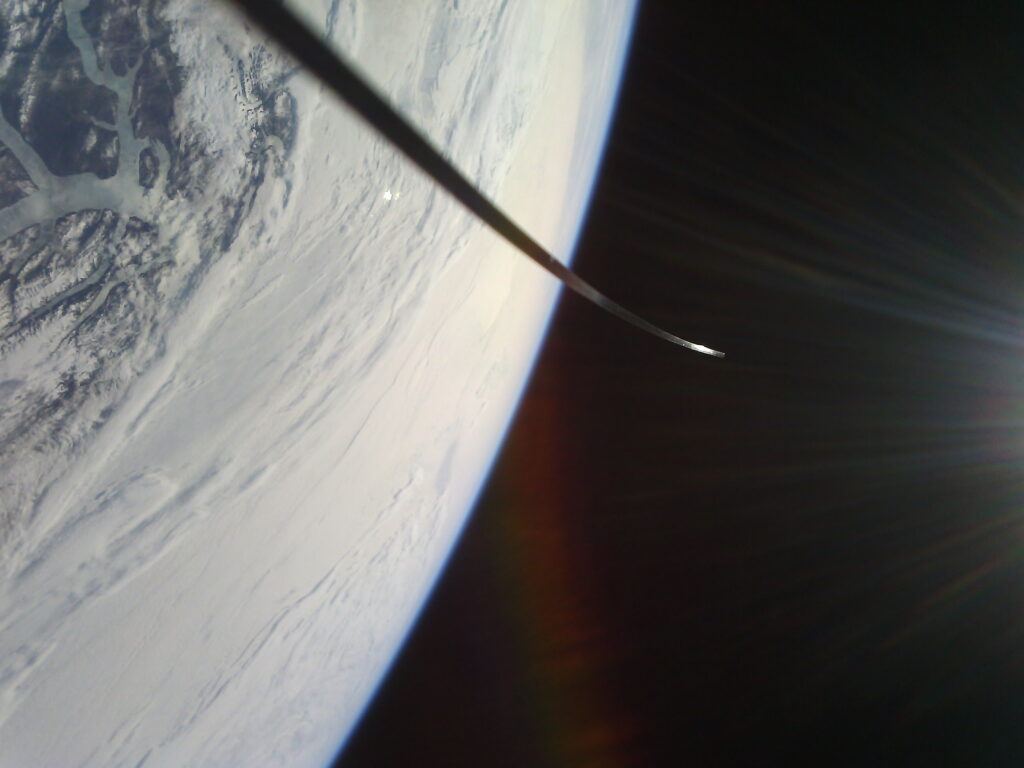
\includegraphics[width=9.5cm]{figures/stf-1-ex6.jpg}
        \end{center}
    \end{figure}

\end{frame}

    \section{Preliminary Design}

        %
% design.tex
%
% Copyright (C) 2022 by SpaceLab.
%
% Camera Payload Preliminary Design Review
%
% This work is licensed under the Creative Commons Attribution-ShareAlike 4.0
% International License. To view a copy of this license,
% visit http://creativecommons.org/licenses/by-sa/4.0/.
%

%
% \brief Design slides.
%
% \author Gabriel Mariano Marcelino <gabriel.mm8@gmail.com>
% \author Vitória Beatriz Bianchin <vitoriabbianchin@gmail.com>
% \author Caique Sales de Miranda Gomes <kiqsmg@gmail.com>
%
% \version 0.1.0
%
% \date 2022/06/24
%


\begin{frame}{Specifications}

    \begin{itemize}
        \item \textbf{Sensor type}: RGB
        \item \textbf{Pixel size}: 2,2 $\times$ 2,2 $\mu$m
        \item \textbf{Max. Resolution}: 1600 $\times$ 1200 px
        \item \textbf{Field of View (FoV)}: \textcolor{red}{TBD}
        \item \textbf{Storage}: 16 MB (Flash NAND)
        \item \textbf{Power supply}: 3V3 @ \textcolor{red}{TBD} mA
        \item \textbf{Interfaces}:
            \begin{itemize}
                \item \textbf{Control/Data}: SPI and/or CAN
                \item \textbf{Debug}: UART
                \item \textbf{Programming}: JTAG
            \end{itemize}
    \end{itemize}

\end{frame}

% #########################################################################
% #########################################################################

\begin{frame}{Electrical Block Diagram}

    \begin{figure}[!ht]
        \begin{center}
            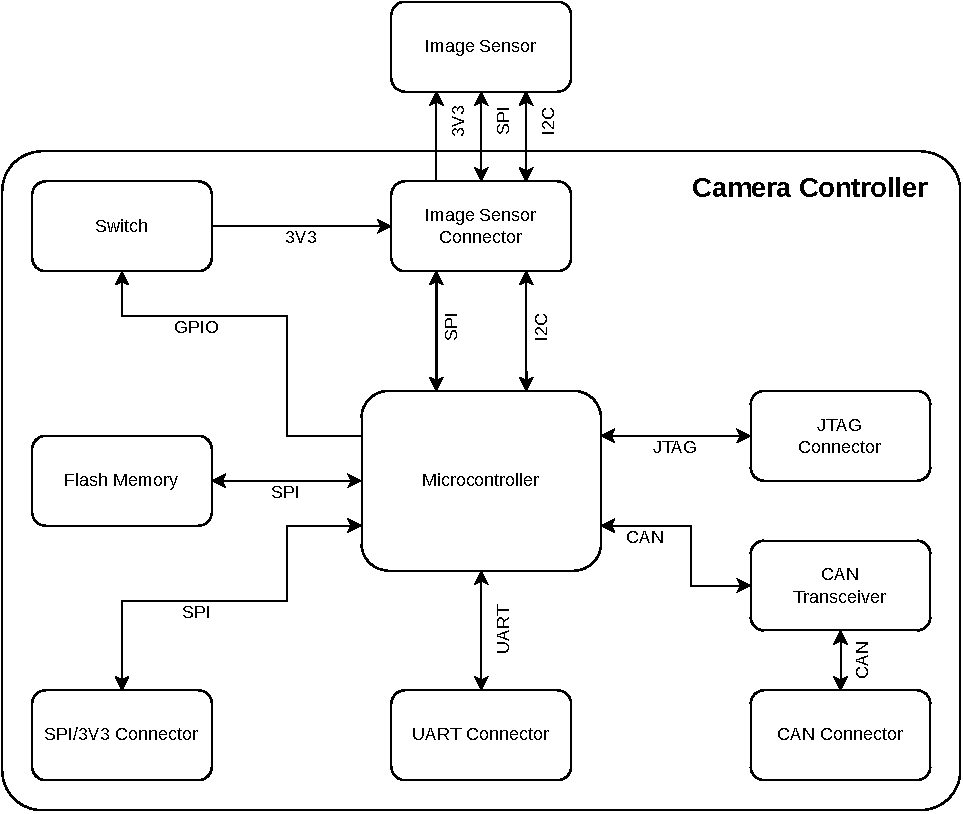
\includegraphics[scale=0.5]{figures/block-diagram}
        \end{center}
    \end{figure}

\end{frame}

% #########################################################################
% #########################################################################

\begin{frame}{Bill Of Materials}

    \begin{table}[!htb]\tiny
        \centering
        \label{tab:bom}
        \begin{tabular}{lL{2cm}cc}
            \toprule[1.5pt]
            \textbf{Component} & \textbf{Description} & \textbf{Partnumber} & \textbf{Quantity} \\
            \midrule
            Microcontroller        & ARM Cortex M3                & STM32F103C8T6        & 1 \\
            Flash Memory           & NOR 128 Mbit                 & W25Q128JVSIM TR      & 1 \\
            Switch                 & Load switch                  & TPS2010AD            & 1 \\
            CAN Transceiver        & CAN transceiver              & TCAN330GD            & 1 \\
            SPI/3V3 Connector      & PicoBlade 6 pin              & 532610671            & 1 \\
            UART Connector         & PicoBlade 3 pin              & 532610371            & 1 \\
            CAN Connector          & PicoBlade 3 pin              & 532610371            & 1 \\
            Image Sensor Connector & Female header 8 pin straight & -                    & 1 \\
            JTAG Connector         & Male header 4 pin angled     & -                    & 1 \\
            Image Sensor Module    & Arducam Mini 2MP Plus        & -                    & 1 \\
            Crystal                & 8 MHz crystal                & ECS-80-10-33-CHN-TR3 & 1 \\
            Lens                   & M12 lens                     & \textcolor{red}{TBD} & 1 \\
            Case                   & Aluminum case                & Custom               & 1 \\
            \bottomrule[1.5pt]
        \end{tabular}
    \end{table}

\end{frame}

% #########################################################################
% #########################################################################

\begin{frame}{Camera Sensor Module}

    \begin{columns}[t]
        \begin{column}[t]{0.6\textwidth}
            \begin{itemize}
                \item Module: \href{https://www.arducam.com/product/arducam-2mp-spi-camera-b0067-arduino/}{\textcolor{blue}{\underline{Arducam Mini 2MP Plus}}}
                \item Image sensor: OV2640
                \item Sensor type: RGB CMOS
                \item Res.: 2 MP (1600 $\times$ 1200 px)
                \item Power supply: 3,3/5 V
                \item Interfaces:
                    \begin{itemize}
                        \item Control: I$^{2}$C
                        \item Data: SPI
                    \end{itemize}
                \item Lens mount: M12
                \item Dimensions: 34 $\times$ 24 mm
            \end{itemize}
        \end{column}
        \begin{column}[t]{0.4\textwidth}
            \vspace{1cm}
            \begin{figure}[!ht]
                \begin{center}
                    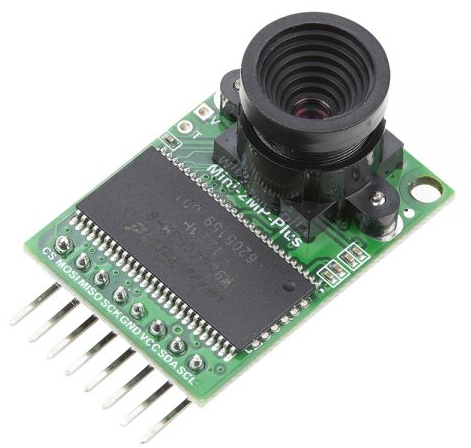
\includegraphics[width=4cm]{figures/arducam-2mp}
                \end{center}
            \end{figure}
        \end{column}
    \end{columns}

\end{frame}

% #########################################################################
% #########################################################################

\begin{frame}{Camera Sensor Module: Architecture}

    \begin{figure}[!ht]
        \begin{center}
            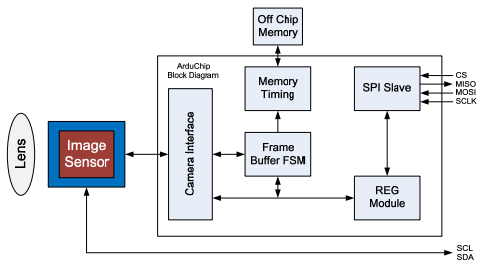
\includegraphics[width=8cm]{figures/arducam-block-diagram}
        \end{center}
    \end{figure}        
    
    \begin{itemize}
        \item ArduChip: FPGA (Lattice)
        \item Off Chip Memory: FIFO
        \item Image Sensor: OmniVision OV2640
    \end{itemize}
                        
\end{frame}             
 
% #########################################################################
% #########################################################################

\begin{frame}{Camera Sensor Module: Dimensions}

    \begin{figure}[!ht]
        \begin{center}
            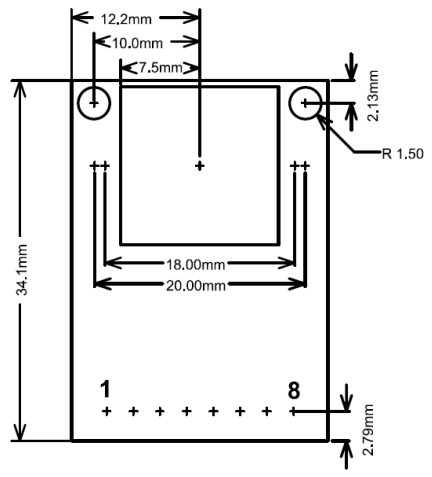
\includegraphics[width=6cm]{figures/arducam-dimensions}
        \end{center}
    \end{figure}        
    
\end{frame}             

% #########################################################################
% #########################################################################

\begin{frame}{Controller}

\textcolor{blue}{Colocar imagem do 3D da placa + resumo das specs. da placa}

\end{frame}

% #########################################################################
% #########################################################################

\begin{frame}{Optic System}

    \begin{itemize}
        \item Mount: M12
        \item FoV: XX$^{\circ}$ \textcolor{red}{TBD}
        \item With IR-filter
        \item Focus: Fixed, infinity
    \end{itemize}

\end{frame}

% #########################################################################
% #########################################################################

\begin{frame}{Mechanical Structure}

\textcolor{blue}{Colocar info e imagens do case de alumínio!!}

\end{frame}

% #########################################################################
% #########################################################################

\begin{frame}{Interface Requirements (ICD)}

\end{frame}

% #########################################################################
% #########################################################################

\begin{frame}{Power Consumption}

    \begin{itemize}
        \item ...
    \end{itemize}

\end{frame}

% #########################################################################
% #########################################################################

\begin{frame}{Dimensions}

    \textcolor{blue}{COLOCAR DESENHO COM DIMENSÕES!!!!}

\end{frame}

% #########################################################################
% #########################################################################

\begin{frame}{Satellite Integration: GOLDS-UFSC}

\textcolor{blue}{Colocar imagens da câmera instalada no GOLDS-UFSC (3D)}

\end{frame}

% #########################################################################
% #########################################################################

\begin{frame}{Firmware}

    \begin{itemize}
        \item OS: FreeRTOS
        \item ...
    \end{itemize}

\end{frame}

% #########################################################################
% #########################################################################

\begin{frame}{Firmware: Development Environment}

    \begin{columns}[t]
        \begin{column}[t]{0.6\textwidth}
            \begin{itemize}
                \vspace{0.4cm}
                \item Hardware: Generic STM32 Cortex-M3 dev kit
                \vspace{0.4cm}
                \item Programmer: ST-Link V2
                \vspace{0.4cm}
                \item Compiler: GCC (arm-none-eabi-XXX)
                \vspace{0.4cm}
                \item Programming tool: \href{https://github.com/stlink-org/stlink}{\textcolor{blue}{\underline{stlink}}}
            \end{itemize}
        \end{column}
        \begin{column}[t]{0.4\textwidth}
            \begin{figure}[!ht]
                \begin{center}
                    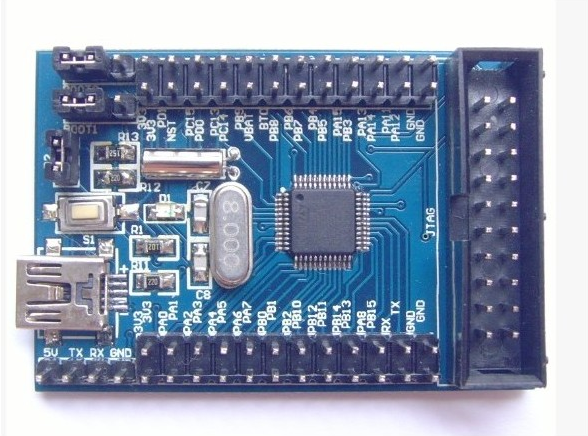
\includegraphics[width=4cm]{figures/stm32-dev-kit}
                \end{center}
            \end{figure}
            \begin{figure}[!ht]
                \begin{center}
                    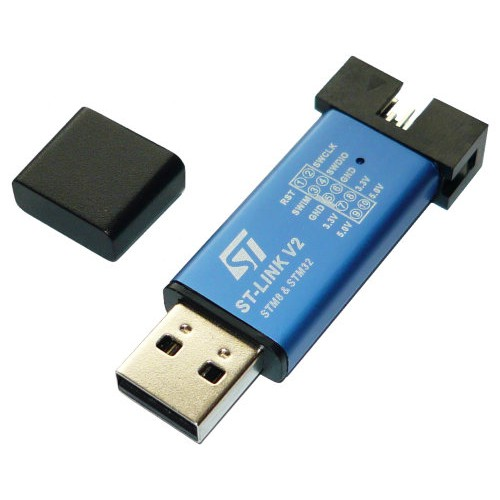
\includegraphics[width=3.5cm]{figures/stlink-v2}
                \end{center}
            \end{figure}
        \end{column}
    \end{columns}
\end{frame}

% #########################################################################
% #########################################################################

\begin{frame}{Firmware: Commands}

\begin{table}[!htb]
    \centering
    \label{tab:commands}
    \begin{tabular}{cll}
        \toprule[1.5pt]
        \textbf{ID} & \textbf{Command} & \textbf{Parameters}\\
        \midrule
        1 & Read ID                 & None \\
        2 & Power On/Off sensor     & 1 or 0 \\
        3 & Take picture            & None \\
        4 & Enable periodic capture & None \\
        5 & Read last picture       & None \\
        6 & Delete last picture     & None \\
        7 & Erase memory            & None \\
        8 & Set parameter           & Parameter ID + Parameter value \\
        9 & Get parameter           & Parameter ID \\
        \bottomrule[1.5pt]
    \end{tabular}
\end{table}

\end{frame}

\begin{frame}{Firmware: Commands}

\begin{table}[!htb]
    \centering
    \label{tab:parameters}
    \begin{tabular}{clll}
        \toprule[1.5pt]
        \textbf{ID} & \textbf{Name} & \textbf{Type} & \textbf{Access} \\
        \midrule
        0 & Module ID                   & uint16 & R\\
        1 & Sensor status               & uint8  & R  \\
        2 & Capture period (in seconds) & uint8  & R/W \\
        4 & Pictures in memory          & uint8  & R/W \\
        \bottomrule[1.5pt]
    \end{tabular}
\end{table}

\end{frame}

    \section{Management}

        %
% management.tex
%
% Copyright (C) 2022 by SpaceLab.
%
% Camera Payload Preliminary Design Review
%
% This work is licensed under the Creative Commons Attribution-ShareAlike 4.0
% International License. To view a copy of this license,
% visit http://creativecommons.org/licenses/by-sa/4.0/.
%

%
% \brief Project management slides.
%
% \author Gabriel Mariano Marcelino <gabriel.mm8@gmail.com>
% \author Vitória Beatriz Bianchin <vitoriabbianchin@gmail.com>
% \author Caique Sales de Miranda Gomes <kiqsmg@gmail.com>
%
% \version 0.1.0
%
% \date 2022/06/24
%


\begin{frame}{Project Management}

    \begin{itemize}
        \item Activities and tasks: GitHub issues/project
        \vspace{0.25cm}
        \item Periodic meetings
        \vspace{0.25cm}
        \item Source files and versioning control: Git/GitHub repository (\href{https://github.com/spacelab-ufsc/camera}{\textcolor{blue}{https://github.com/spacelab-ufsc/slcam}}) with five development branches:
            \begin{itemize}
                \item \textit{dev\_doc}: Documentation
                \item \textit{dev\_hardware}: Hardware project
                \item \textit{dev\_firmware}: Firmware project
                \item \textit{dev\_software}: Software project
                \item \textit{dev\_mechanical}: Mechanical project
            \end{itemize}
    \end{itemize}

\end{frame}

% #########################################################################
% #########################################################################

\begin{frame}{Product Tree}

    \begin{figure}[!ht]
        \begin{center}
            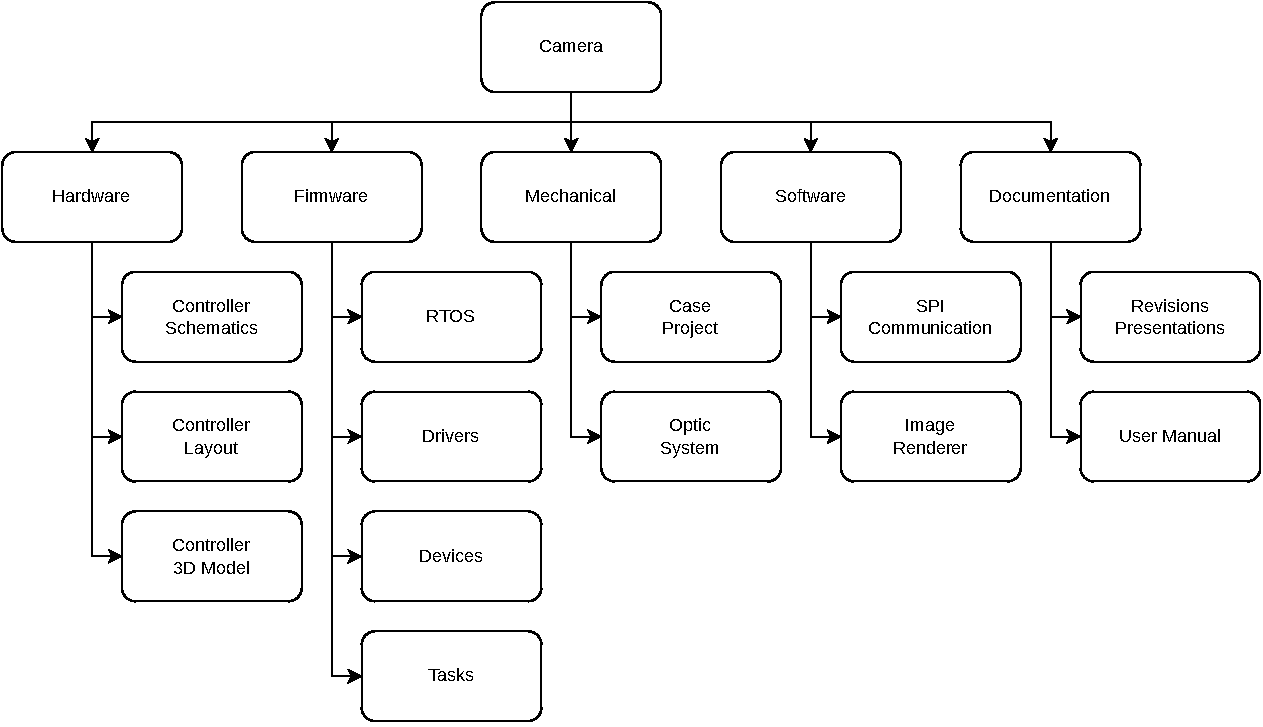
\includegraphics[width=11cm]{figures/product-tree-cam}
        \end{center}
    \end{figure}

\end{frame}

% #########################################################################
% #########################################################################

\begin{frame}{Schedule}

\begin{table}[!htb]\tiny
    \centering
    \label{tab:schedule}
    \begin{tabular}{lC{0.15cm}C{0.15cm}C{0.15cm}C{0.15cm}C{0.15cm}C{0.15cm}C{0.15cm}C{0.15cm}C{0.15cm}C{0.15cm}C{0.15cm}C{0.15cm}C{0.15cm}C{0.15cm}}
        \toprule[1.5pt]
        \multirow{2}{*}{\textbf{Activity}} & \multicolumn{13}{c}{\textbf{Week}} \\
                          & W0 & W1 & W2 & W3 & W4 & W5 & W6 & W7 & W8 & W9 & W10 & W11 & W12 & W13\\
        \midrule
        Project definition            & X &   &   &   &   &   &   &   &   &   &   &   &   &   \\
        Components aquisiton          & X & X & X & X &   &   &   &   &   &   &   &   &   &   \\
        Controller schematics         &   &   & X & X & X &   &   &   &   &   &   &   &   &   \\
        Mechanical structure design   &   &   & X & X & X & X &   &   &   &   &   &   &   &   \\
        \textbf{PDR}                  &   &   &   &   & X &   &   &   &   &   &   &   &   &   \\
        Controller PCB layout         &   &   &   &   &   & X & X & X &   &   &   &   &   &   \\
        Firmware development          &   &   &   &   &   & X & X & X & X & X & X & X &   &   \\
        Test software development     &   &   &   &   &   & X & X & X & X & X & X & X &   &   \\
        Mockup fabrication            &   &   &   &   &   &   &   & X &   &   &   &   &   &   \\
        \textbf{CDR}                  &   &   &   &   &   &   &   &   & X &   &   &   &   &   \\
        Controller PCB fabrication    &   &   &   &   &   &   &   &   & X & X & X & X &   &   \\
        Case fabrication              &   &   &   &   &   &   &   &   & X & X & X & X &   &   \\
        Electrical and firmware tests &   &   &   &   &   &   &   &   &   &   &   &   & X &   \\
        Mechanical integration        &   &   &   &   &   &   &   &   &   &   &   &   & X &   \\
        User manual preparation       &   &   &   &   &   &   &   &   &   &   & X & X & X &   \\
        \textbf{AR}                   &   &   &   &   &   &   &   &   &   &   &   &   &   & X \\
        \bottomrule[1.5pt]
    \end{tabular}
\end{table}

\end{frame}

% #########################################################################
% #########################################################################

\begin{frame}{Team}

\begin{table}[!htb]
    \centering
    \label{tab:team}
    \begin{tabular}{ll}
        \toprule[1.5pt]
        \textbf{Role} & \textbf{Name} \\
        \midrule
        Management/Support                    & Gabriel Mariano Marcelino \\
        Hardware design                       & Vitória Beatriz Bianchin \\
        \multirow{2}{*}{Firmware development} & \textcolor{red}{TBD} \\
                                              & Vitória Beatriz Bianchin \\
        Software development                  & \textcolor{red}{TBD} \\
        Mechanical design                     & Caique Sales de Miranda Gomes \\
        \bottomrule[1.5pt]
    \end{tabular}
\end{table}

\end{frame}

% #########################################################################
% #########################################################################

\begin{frame}{Cost Estimation\footnote{2 units.}}

\begin{table}[!htb]\scriptsize
    \centering
    \label{tab:cost-estimation}
    \begin{tabular}{lccc}
        \toprule[1.5pt]
        \textbf{Item} & \textbf{Unit (US\$)} & \textbf{Quantity} & \textbf{Total (US\$)} \\
        \midrule
        Arducam Mini 2MP Plus & 25,99 & 2  & 51,98 \\
        Lens                  & 7,99 \textcolor{red}{TBC} & 2  & 15,98 \\
        STM32 dev kit         & 2,50  & 2  & 5,00 \\
        STM32F103C8T6         & 7,31  & 2  & 14,62 \\
        W25Q128JVSIM          & 1,95  & 2  & 3,90 \\
        TPS2010AD             & 2,96  & 2  & 5,92 \\
        TCAN330GD             & 3,89  & 2  & 7,78 \\
        532610671             & 0,81  & 2  & 1,62 \\
        532610371             & 0,76  & 4  & 3,04 \\
        ECS-80-10-33-CHN-TR3  & 0,69  & 2  & 1,38 \\
        Passive components    & 2,00  & 1  & 2,00 \\
        PCB                   & 0,20  & 10 & 2,00 \\
        Case                  & 30 \textcolor{red}{TBC} & 2  & 60 \\
        \midrule
        Total          & \multicolumn{3}{c}{US\$175,92\footnote{Prices in June 2022, without delivery rates or taxes.}} \\
        \bottomrule[1.5pt]
    \end{tabular}
\end{table}

\end{frame}

    \sectionpic{Thanks!}{figures/brazil-south.jpeg}

\end{document}
